\documentclass[]{article}

\usepackage{amsmath}
\usepackage{amssymb}
\DeclareMathOperator*{\argmax}{arg\,max}
\DeclareMathOperator*{\argmin}{arg\,min}

\usepackage{setspace}
\linespread{1.5}
\usepackage[margin=1in]{geometry}

\usepackage{graphicx}

%opening
\title{}
\author{}

\begin{document}
%\title{A Machine Learning Framework for Simultaneous Domain Adaption, Map Estimation, and Representation Learning for Datasets with Domain Variability}
\title{Feature Learning for Datasets with Domain Variability}
\author{Michael Wilson}
\date{November 2022}
\maketitle

\begin{abstract}
We present a general machine learning framework for simultaneous alignment, feature learning, and classification. We present results on real and simulated data.  
\end{abstract}

\section{Unimodal Data}

\subsection{Berkeley Growth Data}

For our first example, we consider classifying the Berkeley Growth Curves into male and female. This is not intended to be the optimal machine learning pipeline for this data set; on the contrary, it is intended to be a simple illustration of a much more general pipeline that can be applied to any data set with domain variability. With that in mind, our pipeline for this data set will be as follows;\\

\noindent
1) Multiple Alignment\\
2) Select extrema of mean function as features\\
3) Use 1-cut decision trees to determine maximally informative features\\
4) SVM with Gaussian Kernel for Classification\\

Our first step is to perform multiple alignment on our functions, and calculate a (centered) shape mean for the data. Given our shape mean, there are many ways to perform feature extraction. For simplicity, we will just treat the function values at time points corresponding to the local extrema of our shape mean as our features. The results of these steps are presented in Figure $\ref{aligned function}$. 

After alignment, our feature extraction method finds 12 features, denoted with black dots in Figure $\ref{aligned function}$. Now we wish to determine which of our features are informative for classification. There are many ways to measure the informativeness of a feature, with the simple 1-cut decision tree being among the simplest. Thus, our next step is to select a subset of maximally informative features, defined in terms of the Leave-One-Out classification accuracy of 1-cut decision trees built on each individual feature. The results of these models are presented in Table \ref{feature_LOO}.

\begin{center}
	\begin{figure}[h!]
		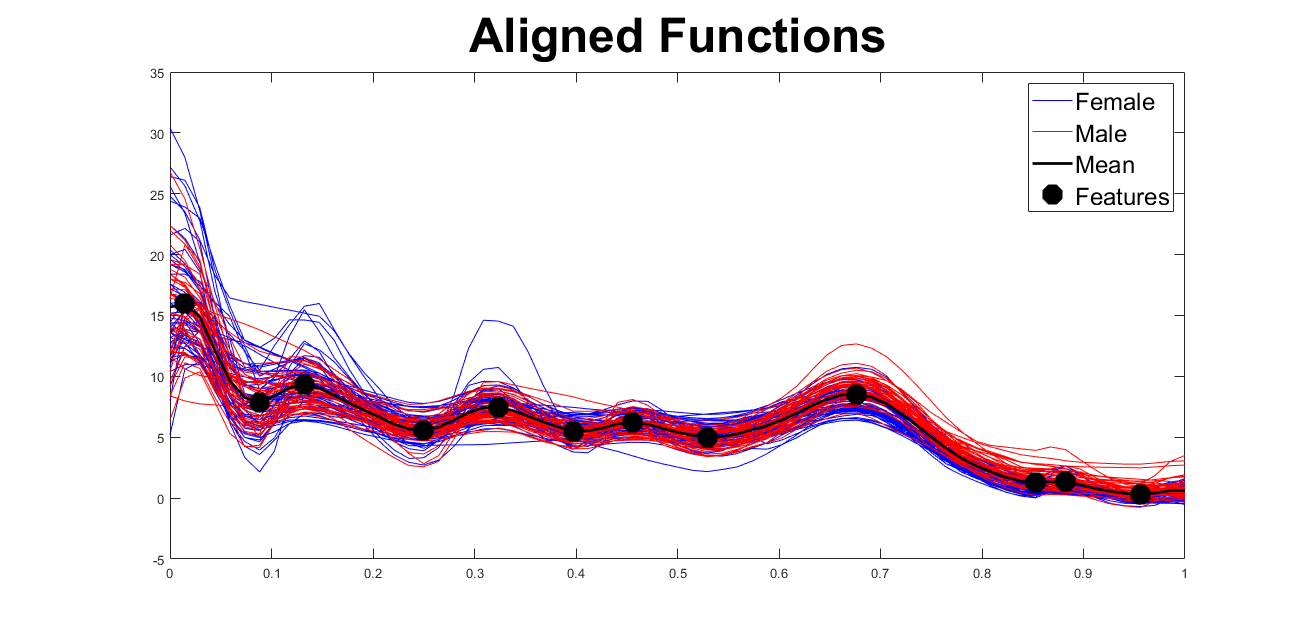
\includegraphics[width = \linewidth]{./Aligned Functions.png}
		\caption{This is the caption}
		\label{aligned function}
	\end{figure}
\end{center}


\begin{table}
	\begin{tabular}{|c|c|c|c|c|c|c|c|c|c|c|c|c|c|c|}
		\hline
		\text{Feature:}& 1 & 2 & 3 & 4 & 5 & 6 & 7 & 8 & 9 & 10 & 11 & 12\\
		\hline
		\text{1-cut Tree }&  &  &  &  &  &  &  &  &  &  &  & \\ 
		\text{LOO Accuracy:}& 0.52 & 0.58 & 0.58 & 0.52 & 0.48 & 0.55 & 0.57 & 0.58 & 0.78 & 0.70 & 0.62 & 0.72\\ 
		\hline
	\end{tabular}
	\caption{Even though our feature extraction picks out 12 features, only features 9, 10, and 12 achieve higher than 0.7 percent test set accuracy.}
	\label{feature_LOO}
\end{table}

Given our measure of informativeness, we will now select some number of features to build our classifier on. We could combine this step with the previous step, and simply treat the number of features as a hyper parameter, however, the intention of the current approach is to provide simple models built on highly interpretable features. While for this data set it isn't entirely necessary, the simplicity and interpretability are very useful in our analysis of DTMRI data in section $\ref{DTMRI}$.  

In any case, Figure \ref{EX1: classifier plot} shows the results of running a Gaussian Kernel SVM using only features 9 and 12. The model achieves 89.25\% for both training set and Leave-one-out test set accuracy, and between 87.1-89.25\% for 10-fold cross validation. Furthermore, the features are very interpretable; feature 9 might be called an 'early puberty high', while feature 12 might be called a 'late puberty low'. Males tend to have higher growth rates at both of these time points, and a classifier built on these two features gets high classification accuracy. 

It is worth noting that this model performs significantly better than a model built on elastic pairwise distances.   

\begin{center}
	\begin{figure}[h!]
		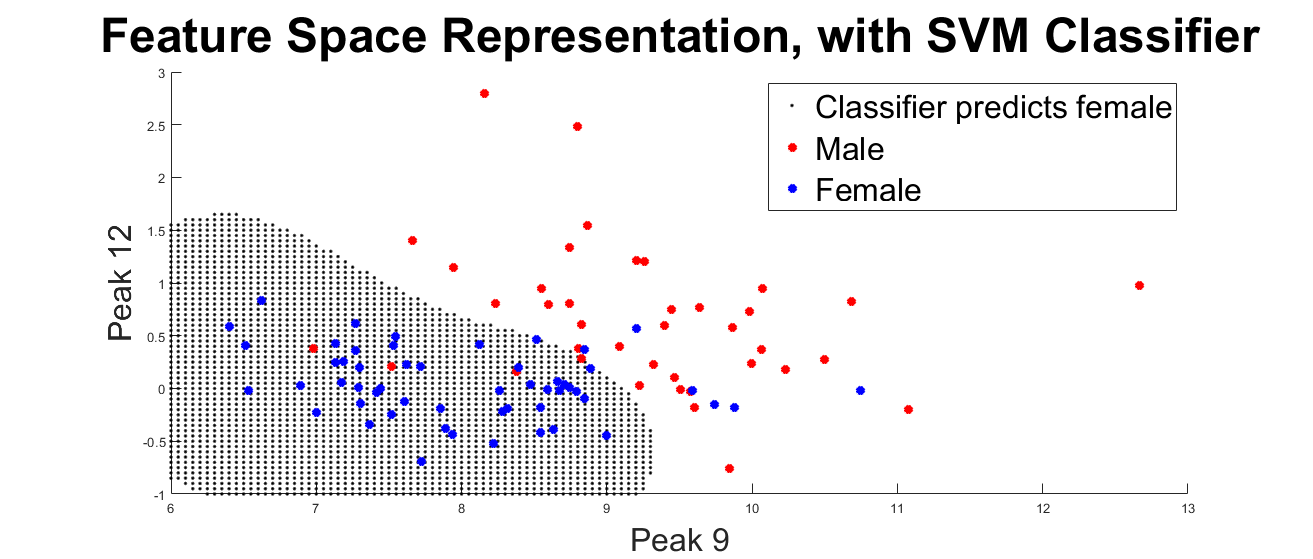
\includegraphics[width = \linewidth]{./Feature Space.png}
		\caption{This is the caption}
		\label{EX1: classifier plot}
	\end{figure}
\end{center}


\newpage

\section{Multi-modal Shape Distribution}

The basic pipeline is as follows;\\

%\noindent
%1) Within-subject Representation Learning\\
%2) Pairwise subject alignment\\
%3) Across-subject Representation Learning \\
%4) Classification\\

\subsection{DTMRI Data}\label{DTMRI}

\end{document}
